
%(BEGIN_QUESTION)
% Copyright 2010, Tony R. Kuphaldt, released under the Creative Commons Attribution License (v 1.0)
% This means you may do almost anything with this work of mine, so long as you give me proper credit

\noindent
{\bf Lab Exercise}

\vskip 5pt

Your task is to build, calibrate, and document a pneumatic system consisting of a pneumatic loop controller connected to a control valve.  If your team's process controller does not have PV and/or SP indicators to calibrate and align, you must build a working process for the controller to regulate.

An additional objective of this lab is to properly cut, bend, and fit metal instrument tubing.  Each student is to bend a length of copper or stainless-steel tubing somewhere in their pneumatic controller/valve system and demonstrate to the instructor that the tubes all fit neatly (right-angle corners, proper offsets, level and plumb).  Instrument tube bending is something of an art, and requires practice to master.

The following table of objectives show what you and your team must complete within the scheduled time for this lab exercise.  Note how some of these objectives are individual, while others are for the team as a whole:

\underbar{Objective completion table:}

% No blank lines allowed between lines of an \halign structure!
% I use comments (%) instead, so that TeX doesn't choke.

$$\vbox{\offinterlineskip
\halign{\strut
\vrule \quad\hfil # \ \hfil & 
\vrule \quad\hfil # \ \hfil & 
\vrule \quad\hfil # \ \hfil & 
\vrule \quad\hfil # \ \hfil & 
\vrule \quad\hfil # \ \hfil & 
\vrule \quad\hfil # \ \hfil & 
\vrule \quad\hfil # \ \hfil \vrule \cr
\noalign{\hrule}
%
% First row
{\bf Performance objective} & {\bf Grading} & {\bf 1} & {\bf 2} & {\bf 3} & {\bf 4} & {\bf Team} \cr
%
\noalign{\hrule}
%
% Another row
Prototype sketch ({\it before building the system!}) & mastery & -- & -- & -- & -- & \cr
%
\noalign{\hrule}
%
% Another row
Final loop diagram and system inspection & mastery & & & & & -- -- -- -- \cr
%
\noalign{\hrule}
%
% Another row
Indicator calibration / working process & mastery & -- & -- & -- & -- &  \cr
%
\noalign{\hrule}
%
% Another row
Demonstration direct and reverse actions & mastery & -- & -- & -- & -- &  \cr
%
\noalign{\hrule}
%
% Another row
Explain proportional control mechanism & mastery & & & & & -- -- -- -- \cr
%
\noalign{\hrule}
%
% Another row
Metal tubing properly fitted & mastery & & & & & -- -- -- -- \cr
%
\noalign{\hrule}
%
% Another row
Lab question: Selection/testing & proportional &  &  &  &  & -- -- -- -- \cr
%
\noalign{\hrule}
%
% Another row
Lab question: Commissioning & proportional &  &  &  &  & -- -- -- -- \cr
%
\noalign{\hrule}
%
% Another row
Lab question: Mental math & proportional &  &  &  &  & -- -- -- -- \cr
%
\noalign{\hrule}
%
% Another row
Lab question: Diagnostics & proportional &  &  &  &  & -- -- -- -- \cr
%
\noalign{\hrule}
%
% Another row
Decommission and lab clean-up & mastery & -- & -- & -- & -- &  \cr
%
\noalign{\hrule}
} % End of \halign 
}$$ % End of \vbox

The only ``proportional'' scoring in this activity are the lab questions, which are answered by each student individually.  A listing of potential lab questions are shown at the end of this worksheet question.  The lab questions are intended to guide your labwork as much as they are intended to measure your comprehension, and as such the instructor may ask these questions of your team day by day, rather than all at once (on a single day).

\vskip 10pt

{\bf It is essential that your team plans ahead what to accomplish each day.  A short (10 minute) team meeting at the beginning of each lab session is a good way to do this, reviewing what's already been done, what's left to do, and what assessments you should be ready for.  There is a lot of work involved with building, documenting, and troubleshooting these working instrument systems!}

As you and your team work on this system, you will invariably encounter problems.  You should always attempt to solve these problems as a team before requesting instructor assistance.  If you still require instructor assistance, write your team's color on the lab whiteboard with a brief description of what you need help on.  The instructor will meet with each team in order they appear on the whiteboard to address these problems.

$$\includegraphics[width=15.5cm]{i01495x01.eps}$$






\vfil \eject

\noindent
{\bf Lab Exercise -- selecting components and planning the system}

\vskip 5pt

One of the most common problems students encounter when building any working system, whether it be a circuit on a solderless breadboard or an instrument loop spanning an entire room, is properly connecting and configuring all components.  An unfortunate tendency among most students is to simply start connecting parts together, essentially designing the system as they go.  This usually leads to improperly-connected components and non-functioning systems, sometimes with the result of destroying components due to those improper connections!

An alternative approach is to plan ahead by designing the system before constructing it.  This is easily done by sketching a diagram showing how all the components should interconnect, then analyzing that diagram and making changes before connecting anything together.  When done as a team, this step ensures everyone is aware of how the system should work, and how it should go together.  The resulting ``prototype'' diagram need not be complex in detail, but it should be detailed enough for anyone to see which component terminals (and ports) connect to terminals and ports of other devices in the system.  For example, your team's prototype sketch should be clear enough to determine all DC electrical components will have the correct polarities.  If your proposed system contains a significant amount of plumbing (pipes and tubes), your prototype sketch should show all those connections as well.

\vskip 10pt

Your first step should be selecting both a control valve and a pneumatic controller to use in building your system.  Note that because this will be a completely {\it pneumatic} system, there is no need for an I/P converter or an electronic valve positioner.  The controller's output tube will connect either directly to the valve's actuating diaphragm, or to the signal input on a pneumatic positioner.  If your controller has PV and SP indicators, I recommend you choose a large control valve such as one of the Fisher E-body valves in the lab.  If your controller does {\it not} have a PV and SP indicator to calibrate, you should choose a small control valve (e.g. Research Control) to build a real working pressure-control process since you will need to do this in lieu of calibrating PV/SP indicators.

The next step should be finding appropriate documentation for your pneumatic controller.  Nearly every instrument in the lab is documented electronically at the manufacturer's website, so your best resource is the Internet (and/or your Instrumentation Reference where a variety of instrument manuals have been downloaded for you).  Use this documentation to identify how to properly install, tube, and calibrate the controller.  Your instructor will check to see you have located and are familiar with the equipment manual(s).

After locating a suitable controller and its associated documentation, you should qualitatively test it prior to installing it in your system.  This entails applying a pneumatic signal pressure to the PV input with the controller in automatic mode and checking to see that the pneumatic output varies as the input is varied.  If the controller fails to respond properly, notify the instructor and then tag it with a label explaining what it does (or what it fails to do).  This test is best done with the controller's ``integral'' and ``derivative'' actions (if so equipped) set to minimum.  For derivative, this means zero minutes.  For integral, this means maximum minutes per repeat (or minimum repeats per minute).  

\vskip 10pt

Your team's prototype sketch is so important that the instructor will demand you provide this plan before any construction on your team's working system begins.  {\it Any team found constructing their system without a verified plan will be ordered to cease construction and not resume until a prototype plan has been drafted and approved!}  Each member on the team should have ready access to this plan (ideally possessing their own copy of the plan) throughout the construction process.  Prototype design sketching is a skill and a habit you should cultivate in school and take with you in your new career.

\vskip 10pt

{\bf Planning a functioning system should take no more than an hour if the team is working efficiently, and will save you hours of frustration (and possible component destruction!).}






\vfil \eject

\noindent
{\bf Lab Exercise -- building the system}

\vskip 5pt

The Instrumentation lab is set up to facilitate the construction of working pneumatic instrument ``loops,'' with a pneumatic controller panel and ``racks'' set up with 2-inch vertical pipes for attaching field-mounted pneumatic controllers (e.g. Fisher MultiTrol, Foxboro 43).

After getting your prototype sketch approved by the instructor, you are cleared to begin building your system.  Your pneumatic controller may be pre-mounted in a panel, or it may be a field-mounted controller designed to attach to a 2-inch pipe using a special bracket and U-bolts.  These brackets and U-bolts are located in the instrument storage area.

Finally, your pneumatic system needs to have a loop number, so all instruments may be properly labeled.  This loop number needs to be unique, so that another team does not label their instruments and cables the same as yours.  One way to make your loop number unique is to use the equivalent resistor color-code value for your team's color in the loop number.  For example, if you are the ``Red'' team, your loop number could be ``2''. 

\vskip 10pt

{\bf Common mistakes:}

\begin{itemize}
\item{} Neglecting to consult the manufacturer's documentation for field instruments (e.g. how to tube them, how to calibrate them).
\item{} Mounting the field instrument(s) in awkward positions, making it difficult to reach connections or to remove covers when installed.
\item{} Improper pipe/tube fitting installation (e.g. trying to thread tube fittings into pipe fittings and vice-versa).
\item{} Students working on portions of the system in isolation, not sharing with their teammates what they did and how.  It is important that the whole team learns all aspects of their system!
\end{itemize}

\vskip 10pt

{\bf Building a functioning system should take no more than one full lab session (3 hours) if all components are readily available and the team is working efficiently!}





\vfil \eject

\noindent
{\bf Lab Exercise -- documenting the system}

\vskip 5pt

Each student must sketch their own {\it loop diagram} for their team's system, following proper ISA conventions.  Sample loop diagrams are shown in the next question in this worksheet.  These loop diagrams must be {\it comprehensive} and {\it detailed}, showing every tube connection, every signal tube, every tube fitting, range points, etc.  The principle to keep in mind here is to make the loop diagram so complete and unambiguous that anyone can follow it to see what connects to what, even someone unfamiliar with industrial instrumentation.  In industry, loops are often constructed by contract personnel with limited understanding of how the system is supposed to function.  The loop diagrams they follow must be so complete that they will be able to connect everything properly without necessarily understanding how it is supposed to work.

Every instrument and every tube in your loop needs to be properly labeled with an ISA-standard tag number.  An easy way to do this is to wrap a short piece of masking tape around each cable (and placed on each instrument) then writing on that masking tape with a permanent marker.  Although no industry standard exists for labeling signal cables, a good recommendation is to label each two-wire cable with the tag number of the field instrument it goes to.  Thus, every length of two-wire cable in a pressure transmitter circuit should be labeled ``PT-$x$'' (where ``$x$'' is the loop number), every flow control valve should be labeled ``FV-$x$'', etc.  Remember that the entire loop is defined by the process variable it measures: if the PV is {\it temperature} then the transmitter with be a {\it T}T, the control valve will be a {\it T}V, the controller with be a {\it T}C, etc.

When your entire team is finished drafting your individual loop diagrams, call the instructor to do an inspection of the loop.  Here, the instructor will have students take turns going through the entire loop, with the other students checking their diagrams for errors and omissions along the way.  During this time the instructor will also inspect the quality of the installation, identifying problems such as frayed wires, improperly crimped terminals, poor cable routing, missing labels, lack of wire duct covers, etc.  The team must correct all identified errors in order to receive credit for their system.  

After successfully passing the inspection, each team member needs to place their loop diagram in the diagram holder located in the middle of the lab behind the main control panel.  When it comes time to troubleshoot another team's system, this is where you will go to find a loop diagram for that system!

\vskip 10pt

{\bf Common mistakes:}

\begin{itemize}
\item{} Forgetting to label all signal tubes (see example loop diagrams).
\item{} Forgetting to label all field instruments with their own tag names (e.g. PC-83).
\item{} Forgetting to note all pneumatic signal port labels on the controller and valve.
\item{} Forgetting to put your name on the loop diagram!
\item{} Basing your diagram off of a team-mate's diagram, rather than closely inspecting the system for yourself.
\item{} Not placing loop sheet instruments in the correct orientation (field instruments on the left, control room instruments on the right).
\end{itemize}

\vskip 10pt

{\bf Creating and inspecting accurate loop diagrams should take no more than one full lab session (3 hours) if the team is working efficiently!}





\vfil \eject

\noindent
{\bf Lab Exercise -- indicating controller calibration}

\vskip 5pt

If your team's pneumatic controller is an {\it indicating} controller (i.e. it has PV and SP indicators), the team must calibrate both indicators and perform an alignment procedure to ensure the controller sees no error when PV=SP throughout their ranges.  If your team's controller does not indicate the PV, skip this section and proceed to the next where you will be instructed on building a pressure-control system for your controller to regulate.

As in all cases where an instrument must be calibrated, you will need to check the instrument's response against one or more {\it standards}.  In this case, the ideal standard to use is a {\it test gauge} covering the standard pneumatic range of 3-15 PSI.  This gauge, of course, needs to be more accurate than the instrument (controller) you are calibrating with it, meaning an ordinary pressure gauge will be insufficient for the task.  The required calibration accuracy for the controller's PV indicator is $\pm$ 1\%.

The maintenance manual for your pneumatic controller will show you how to connect air pressure sources and test gauges to the controller for all calibration and alignment procedures.

\filbreak

Document the accuracy of the PV indicator before and after adjustment in this table, at five different points throughout its sensing range.  The ``Applied'' signal is the amount of air pressure you apply to the PV input using an air pressure source and test gauge, and the ``Indicated'' signal is the controller's PV indicating pointer:

% No blank lines allowed between lines of an \halign structure!
% I use comments (%) instead, so that TeX doesn't choke.

$$\vbox{\offinterlineskip
\halign{\strut
\vrule \quad\hfil # \ \hfil & 
\vrule \quad\hfil # \ \hfil & 
\vrule \quad\hfil # \ \hfil \vrule \cr
\noalign{\hrule}
%
% First row
Applied signal & Indicated value (As-Found) & Indicated value (As-left) \cr
%
\noalign{\hrule}
%
% Another row
 &  & \cr
%
\noalign{\hrule}
%
% Another row
 &  & \cr
%
\noalign{\hrule}
%
% Another row
 &  & \cr
%
\noalign{\hrule}
%
% Another row
 &  & \cr
%
\noalign{\hrule}
%
% Another row
 &  & \cr
%
\noalign{\hrule}
} % End of \halign 
}$$ % End of \vbox

When finished calibrating your team's controller, be sure to place a calibration tag on it showing the range and the date it was calibrated.  The first page of this lab exercise has cut-out calibration tags you may tape to the transmitter for this purpose.

\vskip 10pt

{\bf Common mistakes:}

\begin{itemize}
\item{} Neglecting to follow manufacturer's instructions for calibrating and aligning the indicators.
\item{} Failing to closely inspect pressure regulators before connecting them to an air source (e.g. connecting the air supply to the ``out'' port)
\item{} Improper pipe/tube fitting installation (e.g. trying to thread tube fittings into pipe fittings and vice-versa).
\item{} Neglecting to place a calibration tag on the controller after calibrating it.
\end{itemize}

\vskip 10pt

{\bf Calibrating your controller should take no more than one full lab session (3 hours) if the team is working efficiently!}



\vfil \eject

\noindent
{\bf Lab Exercise -- building a pressure control system}

\vskip 5pt

If your team's pneumatic controller does not have either PV or SP indicators to calibrate and align, you must build a real pressure control system for your controller to regulate.  This makes the lab exercises equitable between different teams regardless of controller model, since the tasks of calibrating and aligning PV/SP indicators can be time-consuming.

\vskip 10pt

An easy way to build a real system that is easily controlled by a pneumatic loop controller is to use a set of hand valves and capacity tanks to create a second-order lag system, whereby the second tank's pressure may be directly read by the pneumatic controller as a 3-15 PSI signal:

$$\includegraphics[width=15.5cm]{i01495x02.eps}$$

The required controller gain setting will depend on the size ($C_v$) of the control valve, the tank volumes, and the positions of the hand valves.  The two series hand valves change process lag times, while the two vent valves serve as process loads.  Large tank volumes produce long lag times, so be careful not to connect capacity tanks too large.  Something around the size of a half-gallon each works quite well.  In a pinch, a single tank will suffice, but a pair of tanks does create more interesting control behavior.

To make the simulated process even more interesting, you may wish to connect an electronic pressure transmitter to the PV tube and have it send its signal to an inexpensive data acquisition unit (or a chart recorder) to record the PV over time as you make setpoint, gain, and process valve adjustments.

\vskip 10pt

Demonstrating the system in stable automatic control will be considered equivalent for the credit other teams receive calibrating and aligning their pneumatic controller indicators.



\vfil \eject

\noindent
{\bf Lab Exercise -- instrument tube fitting}

\vskip 5pt

An additional objective of this lab is learn how to properly bend instrument tubing.  Each student is to bend a length of copper or stainless-steel tubing somewhere in their pneumatic controller/valve system and demonstrate to the instructor that the tubes all fit neatly (right-angle corners, proper offsets, no gradual bends, all straight sections level and plumb).  Instrument tube bending is something of an art, and requires practice to master!

An ideal application for tube bending are the lines to and from a valve positioner, assuming your valve uses a positioner.  If not, and you are building a working process (for a pneumatic controller lacking PV and SP indication), you may bend and fit tubes connecting the process vessel(s) to other parts of the system.

Rolls of soft copper tubing will be provided by the instructor to use in this lab exercise.  Each student's tube run should be relatively short (less than 2 feet) in order to conserve the amount of tubing used.  Expect to make at least two attempts when fitting your tube run!

Videos are available on the BTC Instrumentation YouTube channel showing some of the basic procedures of tube cutting, bending, and compression fitting make-up.  Each team has a professional-quality 1/4-inch tube bender in their locker, to be used for this exercise.

Your Instrumentation Reference also contains manuals from both Swagelok and Parker describing how instrument tube fittings work, and how to properly fit tubing.

\vskip 10pt

{\bf Common mistakes:}

\begin{itemize}
\item{} Applying Teflon tape or other sealant to tube fitting threads (not necessary!).
\item{} Forgetting to apply Teflon tape or other sealant to pipe fitting threads (necessary!).
\item{} Throwing away used tube fittings when done with the job.  Remember than although tube {\it ferrules} cannot be re-used, the nuts and fitting bodies can!
\item{} Over-tightening compression fittings (only 1-1/4 turns past initial contact are necessary when {\it first} ``making-up'' the tube connection!).  When re-making tube connections, you need only ``snug'' the nut, not re-swage with another 1-1/4 turns!
\item{} Trying to straighten a piece of tubing that has already been bent.
\end{itemize}







\vfil \eject

\noindent
{\bf Lab questions}

\vskip 5pt

\begin{itemize}
\item{} {\bf Selection and Initial Testing}
\item{} Locate the controller's restriction (orifice) and explain the purpose of it
\item{} Locate the controller's baffle/nozzle assembly and explain the purpose of it
\item{} Explain (step by step) how to secure a working control loop to calibrate the process transmitter without affecting the process
\item{} Explain (step by step) how to secure a working control loop to stroke and calibrate the control valve without affecting the process
\item{} Identify the preferred tools (in order) to use when connecting tube fitting components: open-end wrench, box-end wrench, pliers, adjustable wrench
\item{} Demonstrate how to properly use an air pump as pressure source to simulate a PV signal input to a pneumatic controller
\end{itemize}

\filbreak

\begin{itemize}
\item{} {\bf Commissioning and Documentation}
\item{} Demonstrate how to isolate potentially hazardous energy in your system ({\it lock-out, tag-out}) and also how to safely verify the energy has been isolated prior to commencing work on the system
\item{} Explain how a {\it tube fitting} seals against fluid leaks
\item{} Explain how a tapered-thread {\it pipe fitting} seals against fluid leaks
\item{} Identify and explain how large signal tube volumes degrade the performance of pneumatic instruments
\item{} Explain how your controller's variable gain mechanism works, and demonstrate its adjustment
\item{} Explain and demonstrate how to switch your controller between direct and reverse control modes
\item{} Explain how to configure your controller to exhibit {\it on/off} (``bang-bang'') control
\item{} Explain where and how PV and SP values are compared (subtracted) in the controller mechanism, since we know all proportional controllers respond to the {\it difference} between PV and SP
\item{} Explain how to safely select a gain value (proportional band) suitable for controlling a live process (i.e. outline a tuning procedure that will not unduly upset the process being controlled)
\end{itemize}

\filbreak

\begin{itemize}
\item{} {\bf Mental math} (no calculator allowed!)
\item{} Convert a gain value into a proportional band value
\item{} Convert a proportional band value into a gain value
\item{} Convert between different pressure units, without relying on the use of a reference for conversion factors (i.e. you must commit the major conversion factors to memory)
\item{} Calculate the pneumatic signal pressure (3-15 PSI range) corresponding to a given percentage value
\item{} Calculate the percentage value corresponding to a given pneumatic signal pressure (3-15 PSI range)
\end{itemize}

\filbreak

\begin{itemize}
\item{} {\bf Diagnostics}
\item{} ``Virtual Troubleshooting'' -- referencing their system's diagram(s), students propose diagnostic tests (e.g. ask the instructor what a meter would measure when connected between specified points; ask the instructor how the system responds if test points are jumpered) while the instructor replies according to how the system would behave if it were faulted.  Students try to determine the nature and location of the fault based on the results of their own diagnostic tests.
\item{} Determine whether or not a given diagnostic test will provide useful information, given a set of symptoms exhibited by a failed system
\item{} Identify at least two plausible faults given the results of a diagnostic test and a set of symptoms exhibited by a failed system
\end{itemize}



\vfil \eject

\noindent
{\bf Lab Exercise -- decommissioning and clean-up}

\vskip 5pt

The final step of this lab exercise is to decommission your team's entire system and re-stock certain components back to their proper storage locations, the purpose of which being to prepare the lab for the next lab exercise.  Remove your system documentation (e.g. loop diagram) from the common holding area, either discarding it or keeping it for your own records.  Also, remove instrument tag labels (e.g. FT-101) from instruments and from cables.  Perform general clean-up of your lab space, disposing of all trash, placing all tools back in their proper storage locations, sweeping up bits of wire off the floor and out of junction boxes, etc.

\vskip 10pt

\indent
{\bf Leave the following components in place, mounted on the racks:}

\begin{itemize}
\item{} Large control valves and positioners
\item{} I/P transducers
\item{} Large electric motors
\item{} Large variable-frequency drive (VFD) units
\item{} Cables inside conduit interconnecting junction boxes together
\item{} Pipe and tube fittings (do not unscrew pipe threads)
\item{} Supply air pressure regulators
\end{itemize}

\vskip 10pt

\indent
{\bf Return the following components to their proper storage locations:}

\begin{itemize}
\item{} Sensing elements (e.g. thermocouples, pH probes, etc.)
\item{} Process transmitters
\item{} ``Jumper'' cables used to connect terminal blocks within a single junction box
\item{} Plastic tubing and tube fittings (disconnect compression-style tube fittings)
\item{} Power cables and extension cords
\item{} Adjustment (loading station) air pressure regulators
\end{itemize}

\vskip 10pt

Finally, you shall return any control system components to their original (factory default) configurations.  This includes controller PID settings, function block programs, input signal ranges, etc.



\underbar{file i01495}
%(END_QUESTION)





%(BEGIN_ANSWER)


%(END_ANSWER)





%(BEGIN_NOTES)

The same basic ``simulated process'' idea may be applied to an electronic controller, using an I/P as the final control element to send compressed air to a set of capacity tanks, and using an electronic pressure transmitter to measure the last tank's pressure and report it as the PV.

\vskip 20pt

\noindent
{\bf Loop diagrams / inspections:}

I strongly recommend checking off students' loop diagrams while you inspect their loop (checking for secure wiring, proper tubing, good conduit installation, etc.) with them.  Have all team members take you on a ``tour'' of their completed loop, with each team member explaining a different portion of the loop you select while using their own loop diagram as a guide.  While a student is explaining their section of the loop, you can check the other students' loop diagrams for accuracy.  This not only saves time by consolidating the tasks of loop inspection and loop diagram verification, but it also ensures students can actually relate their loop diagrams to the loop they have built and articulate that understanding to you.

%INDEX% Lab exercise, pneumatic controller

%(END_NOTES)


